% $Id: system.tex,v 1.7 2006/09/06 19:09:21 borning Exp $

\section {System Design and Implementation process}
\label{sec:system-design}

\subsection{System Design}

The system can be divided into three components: The mechanism that allows
the user to make requests, the mechanism that manages the requests once
they have been submitted; and the mechanism that actually generates the
indicators and their respective visualizations.  A general overview of the
system can be found in Figure \ref{fig:system}.

%system fig
\begin{figure*}
\centering
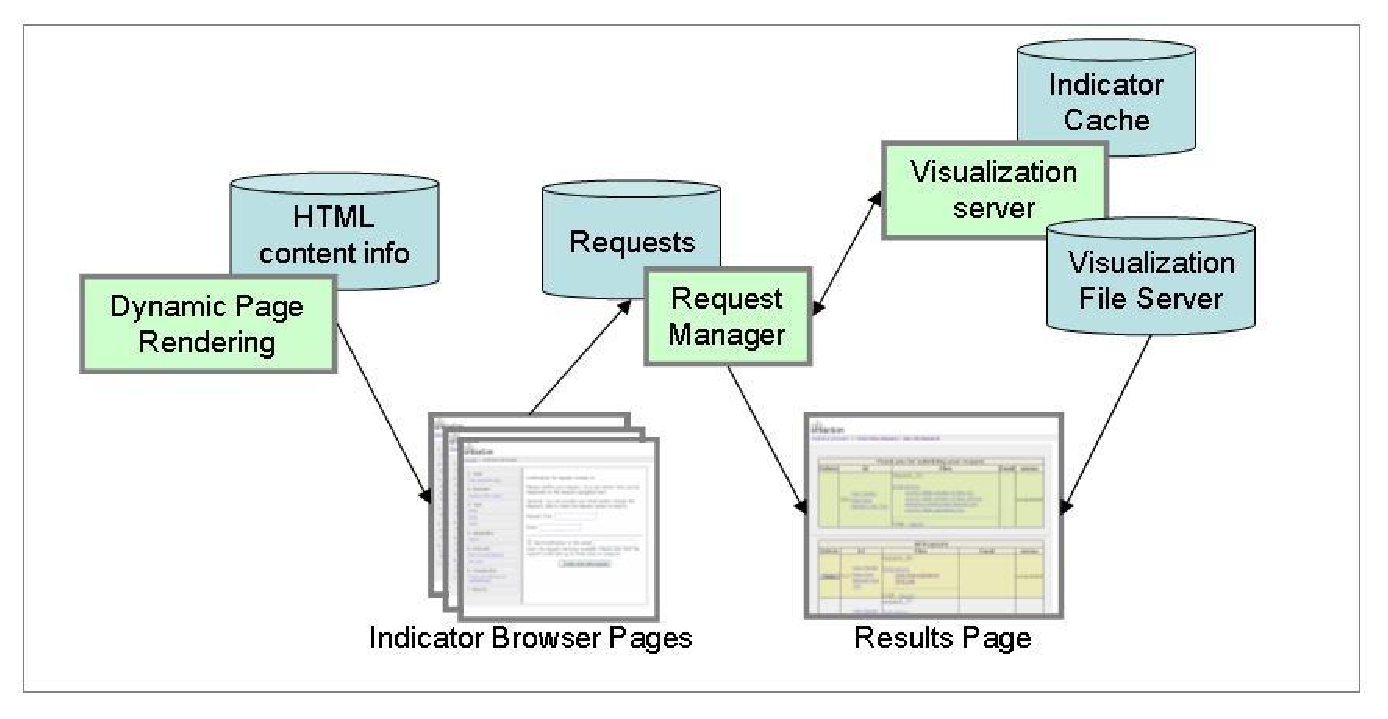
\includegraphics[width =6in]{figs/system}

\caption{\label{fig:system}System Overview.}

\end{figure*}

\subsection{Creating a Visualization Request}

Creating an indicator visualization request is accomplished by allowing the
user to define the request through a sequence of web pages. Each page in
this sequence is channeled through a single CGI page that gathers user
input from the current page, updates the web session, and generates and
displays the subsequent page accordingly. Each web session is determined by
an entry to the {\tt Sessions} table in the Indicator Browser
database. The database not only keeps track of the values that were
selected, but also of the values that are available for future web pages
based on previous selections. For example, suppose we have data for the
year of 2000 and 2001 for Scenario A\@.  If the user selects Scenario A in the
{\tt Scenario} page, then the only options that appear on the {\tt Year}
page are 2000 and 2001. A nice feature of this implementation is
that if one would want to make more options available to the user, it is
only necessary to add one more entry to the corresponding table on the
Indicator Browser database. For example, we are planning to add support for
visualizing the differences between scenarios. If we would want to
allow the users to create these visualizations we would just need to update
the {\tt available tasks} table with information about this new task.

The page rendering is accomplished through a set of HTML templates that
contain general information about how to display a page. A small number of
global templates determine the HTML rendering that pertains to all web
pages on the site, such as the CSS style-sheet link and common navigational
links.  A sidebar template contains the HTML framework for the part of the
web page that displays the session's status (Figure \ref{fig:scenario_full}).
Finally, there is one template per web page that contains more specific
information regarding the rendering of each page. Each web page has its
{\tt Page Builder}, a module that fills in the template blanks and
renders the current state and page of the Indicator Browser.

The {\tt Site Structure} module determines the site's sequence and the
input values and types that one should expect at each page. This provides
flexibility both for the order at which the existing pages are displayed
and for including new pages into the sequence.

Since the rendering of a page usually depends on the previous user
selections, there is a mechanism that determines whether or not there were
changes made to the previous page. If there were changes, and these
invalidate selections made in subsequent pages, all the invalid values are
removed to maintain coherence.

\subsection{Managing Visualization Requests}    

Once the user has selected the scenario run, year(s), indicator(s),
geography, visualization type, request title, option for notification and
email, a request is created and added to the visualization queue. The {\tt
Visualization Manager} is a Windows service hosted at one of UrbanSim's
servers. This service is in charge of managing the request queue by waking
up every so often to:

\begin{itemize}
  \item Send new requests to the {\tt Visualization Service}, the Windows
    service that generates the indicators and their corresponding
    visualizations.
  \item Attempt to complete requests that are being processed by assessing
    whether the visualizations ordered in the request are present in the
    corresponding location in the file system.
  \item Send email to users once the requests have been completed, if the
     users selected to be notified by email. This email contains the
     URL of the web page that displays the indicator visualization
     if the request was completed successfully, and a link
     to the error log otherwise.
  \item Send an email to the Indicator Browser maintainer if there was an
    error processing a request.
\end{itemize}

\subsection{Generating Indicators and Visualizations}

The {\tt Illustrator} is a module that takes in a visualization request,
configures it by adding information that is specific to the Indicator
Browser, and sends it to the {\tt Indicator Factory}. The {\tt Indicator
Factory} is a module that retrieves all the scenario resources, adds them
to the Indicator Browser specific information, creates a file with all this
information, and forks a process for each of the indicators in the
request. This process is called the {\tt Indicator Maker}, which retrieves
this file, all the necessary data from the results of running the scenario,
and computes the values of the indicator.  Once these
values have been computed, the {\tt Indicator Maker} creates a
visualization and saves it both into the scenario cache and into the
Indicator Browser web space, which is one of the specific items of
information required from the {\tt Illustrator} module.


%system fig
%% \begin{figure*}

%% 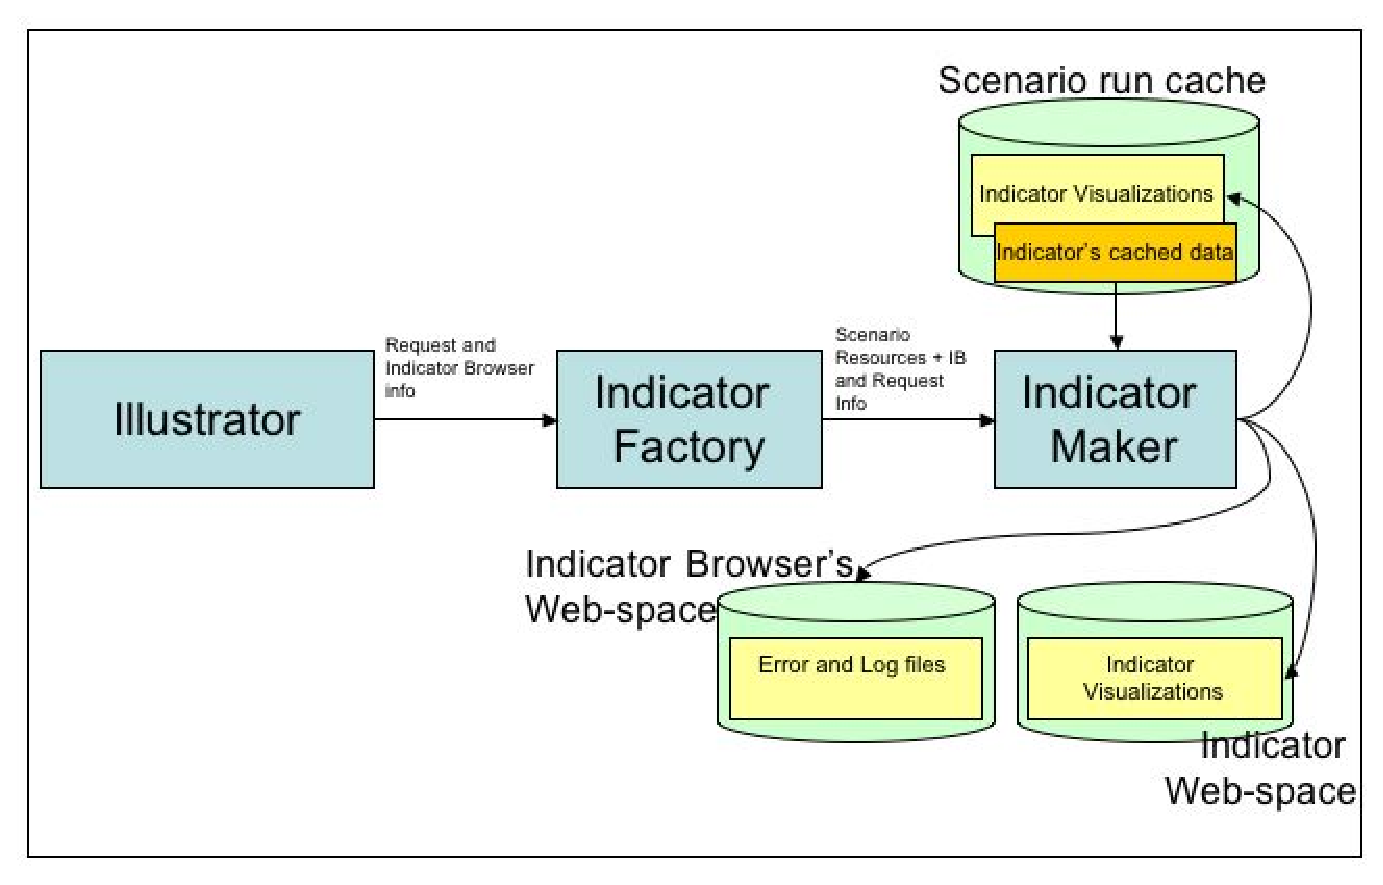
\includegraphics[width =6in]{figs/indgeneration}

%% \caption{\label{fig:indgeneration}Indicator Generation and Visualization}

%% \end{figure*}

% LocalWords:  borning CGI CSS screenshot UrbanSim's run's yaels
